% Supplementary Material of the Ecological Modelling paper. The tables of evaluators, confirmatory tests and
% ensembles are copies of manuscript/pre/tables/ (rows added to the ensembles); the pattern table and the deviations
% come from manuscript/pre/supplement.tex; the ODD is adapted from manuscript/extended/. Figures: scripts/em/em_figs.py.
\documentclass[preprint,12pt,authoryear]{elsarticle}

% Shared preamble of main.tex and supplement.tex (elsarticle, preprint, 12pt, author-year).
\usepackage[utf8]{inputenc}
% No T1 fontenc: cm-super/lmodern are not installed and T1 would embed bitmap (Type 3) fonts.
\usepackage{amsmath,amssymb}
\usepackage{graphicx}
\usepackage{booktabs}
\usepackage{array}
\usepackage{longtable}
\usepackage{xcolor}
\usepackage{xr-hyper}
\usepackage[colorlinks=true,linkcolor=blue!60!black,citecolor=blue!60!black,urlcolor=blue!60!black]{hyperref}
\usepackage{lineno}
\usepackage{adjustbox}
% Itemize bullets from math fonts: \textbullet would pull a bitmap (Type 3) TS1 font into the PDF.
\renewcommand{\labelitemi}{$\bullet$}

\graphicspath{{figs/}}
\biboptions{round,authoryear}

% Model names and recurring symbols.
\newcommand{\Cone}{\textsf{C1}}
\newcommand{\Ctwo}{\textsf{C2}}
\newcommand{\Kg}{K_\gamma}
\newcommand{\eadult}{\epsilon_{\rm ad}}
% Repository and archive.
\newcommand{\repourl}{\url{https://github.com/jfbonder/universe25-abm}}
\newcommand{\zenodo}{\href{https://doi.org/10.5281/zenodo.23111283}{doi:10.5281/zenodo.23111283}}
% Visible placeholder for content the author must supply.
\newcommand{\authorpending}[1]{{\color{red}[AUTHOR: #1]}}
% Let the large figures float near their first citation.
\renewcommand{\topfraction}{0.95}
\renewcommand{\textfraction}{0.05}
\renewcommand{\floatpagefraction}{0.75}
\setcounter{topnumber}{2}
\setcounter{totalnumber}{3}
% Avoid overfull lines in justified text.
\setlength{\emergencystretch}{2em}

\renewcommand{\thetable}{S\arabic{table}}
\renewcommand{\thefigure}{S\arabic{figure}}
\renewcommand{\thesection}{S\arabic{section}}
\renewcommand{\theequation}{S\arabic{equation}}

\journal{Ecological Modelling}

\begin{document}

\begin{frontmatter}
\title{Supplementary Material for ``Simple interaction rules qualitatively reproduce Calhoun's Universe~25: a
pattern-oriented agent-based model of population collapse''}
\author{Juli\'an Fern\'andez Bonder}
\ead{jfbonder@dm.uba.ar}
\affiliation{organization={Departamento de Matemática, FCEN, Universidad de Buenos Aires, and Instituto de
Cálculo, UBA--CONICET},
  city={Buenos Aires},
  country={Argentina}}
\end{frontmatter}

\sloppy
This Supplementary Material contains the patterns and the numbers taken from Calhoun's report, with the dating of
the phases (Section~\ref{supp:patterns}), the full model description following the ODD protocol with the parameter
table (Section~\ref{supp:odd}), the evaluators and the deviations from the preregistration
(Section~\ref{supp:evaluators}), the confirmatory tests (Section~\ref{supp:Q}), the ensembles
(Section~\ref{supp:ensembles}), the robustness analyses and the ablations (Section~\ref{supp:robustness}), the
conditions of the mechanism (Section~\ref{supp:recovery}) and the supplementary videos (Section~\ref{supp:videos}).
The calibration, the phase planes and the full null-model tables are in the extended version in the repository
(\repourl; archived at \zenodo). The adult-recovery sweep, the interventions on non-breeders and on juveniles, the test of mate search, the scaling
of the extinction time and the cohort account of the mechanism are summarised, from archived runs, in
Section~\ref{supp:recovery}.
Model names: \Cone\ is the reference model (core processes and the four social rules R1, R2, AV and R7);
\textsf{C1}$'$ is \Cone\ without crowd aversion; \textsf{C0} is \Cone\ without retreat sites; \Ctwo\ is \Cone\ with
withdrawal driven by the maternal competence at birth.

% ===========================================================================
\section{Patterns and numbers taken from Calhoun's report}
\label{supp:patterns}

Table~\ref{tab:observations-full} lists the seventeen patterns and four anti-patterns with their operational
criteria, and Table~\ref{tab:calhoun-numbers} the numbers taken from the original report \citep{Calhoun1973} with
their conversion to weeks. Every criterion is evaluated per run and returns PASS, MARGINAL, FAIL or NOT APPLICABLE;
an ensemble is summarised by the fraction of PASS runs with a 95\% Wilson interval, and an essential (E) pattern is
reproduced if that fraction is at least 0.8, a desirable (D) pattern if it is at least 0.5 \citep{Grimm2005}. The
primary evaluator replaces $t_{\rm pk}$ by the start of the plateau $t'_{\rm pk}$ (the first week with
$N\ge0.98\,N_{\max}$) in every criterion and, in O5, $t_{B0}$ by the week $t_{B99}$ at which 99\% of the births have
occurred; $f_0$ is measured at $t'_{\rm pk}$ and the crowded class at $m>8$. In the main text O11 is scored at the
end of the sensitive window ($a_w=12$ weeks).

{\small
\begin{longtable}{@{}>{\raggedright\arraybackslash}p{0.065\textwidth}>{\raggedright\arraybackslash}p{0.04\textwidth}>{\raggedright\arraybackslash}p{0.425\textwidth}>{\raggedright\arraybackslash}p{0.36\textwidth}@{}}
\caption{Qualitative patterns (O) and anti-patterns (A). E = essential, D = desirable, X = exploratory.
$^\dagger$O13p is not preregistered (defined after calibration) and enters the primary outcome O17p $=$ O17 $\wedge$
O13p. O17p is strict: a not-applicable essential pattern counts as a failure (except O1--O3 when $N_0>20$, which are
excluded by design), and an evaluation error is never a pass. O17 alone counts not-applicable patterns as passes,
so it is not used as an outcome. $^\ddagger$Consistency check of the design: the pattern follows from the rules by
construction (O12 from R1 and $p_{\rm conc}\propto s_fs_m$; O13p from R7 with $c_R=2$; A4 and the senescent nature of the decline in O8 from $\mu_s=0$, whereas the duration criterion of O8 is not by construction and passes in 0.62 of the \Cone\ runs).
$^\S$Not preregistered: for O4, O10, O10b and O11 the preregistered form also passes in null models (extended version in the repository), and in the primary form O4 and O10 are still generic; O3c and O11 at age $a_w$ were added in the revision. $K_\gamma=m_c|G|$ is the population at which every cell would
sit at the damage threshold; it is not a physical capacity. Page numbers refer to \citep{Calhoun1973}.}
\label{tab:observations-full}\\
\toprule
ID & & Observation in Universe~25 (page) & Operational criterion \\
\midrule
\endfirsthead
\toprule
ID & & Observation (cont.) & Criterion \\
\midrule
\endhead
\bottomrule
\endfoot
O1 & E & 104 days of ``considerable social turmoil'' before the first litters (p.~82) & founder scenario only: $t_{\rm lag}/t_{\rm pk}\in[0.10,0.35]$ (Calhoun $0.19$) \\
O2 & E & Exponential growth, doubling time ``about 55 days'' (p.~83) & $R^2\ge 0.90$ for $\log N$ in the growth window \\
O3 & E & Doubling time rises to ${\approx}145$ days from $N=620$ (pp.~83--84) & $r_B/r_C\ge 2$; phase-C clause O3c$^\S$: $t_D-t_{BC}\ge 0.1\,t_D$ \\
O4 & E$^\S$ & Peak of 2200 versus shelter for 3840, food for 9500 and water for 6144; 20\% of nest boxes empty at the peak (p.~82) & $N_{\rm pk}/K_\gamma\le 0.8$ and empty fraction of cells at the peak $f_0\ge0.10$ \\
O5 & E & Growth ``abruptly ceased'' on day 560; last young surviving weaning born around day 600 (p.~85) & $N(t_{B0})/N_{\rm pk}\ge 0.7$ and $(t_{B0}-t_{\rm pk})/t_{\rm pk}\le 0.5$ \\
O6 & E & No recovery; the demise ``contradicts prior knowledge'' that remnant groups reinitiate growth (p.~85) & no rebound of $\ge 0.1N_{\rm pk}$, including slow regrowth still rising at censoring; birth-rate hysteresis $A_H\le 0.1$ \\
O7 & E & Total demise; last male projected dead on day 1780 (p.~85) & run: extinct by $T$; ensemble: $P_{\rm ext}(T)\ge 0.9$ (Kaplan--Meier) \\
O8 & D$^\ddagger$ & Decline through senescence; mean age of survivors 776 days (p.~85) & $(T_{\rm ext}-t_{\rm pk})/t_{\rm pk}\ge 1$ (Calhoun $\ge 1.84$ observed, $2.2$ projected) \\
O8b & D & Slow initial decline: $N=2056$ on day 736 (p.~83) & $N(1.31\,t_{\rm pk})/N_{\rm pk}\ge 0.8$ (Calhoun $0.93$) \\
O9 & D & 27 survivors (23 F, 4 M), all older than 987 days (p.~83) & no young in the remnant; female fraction $>0.5$ \\
O10 & E$^\S$ & ``death of societal organization by the end of Phase C'' (p.~85) & adult mean competence falls below 0.5 before the peak and stays below it at the peak: $t(\bar s_{\rm ad}<0.5)<t_{\rm pk}$, $\bar s_{\rm ad}(t_{\rm pk})<0.5$ \\
O10b & D$^\S$ & Phase B: 14 functional social groups during growth (days 104--315; pp.~83--84) & adults socially competent during growth: $t(\bar s_{\rm ad}<0.5)\ge 0.5\,t_{\rm pk}$ \\
O11 & E$^\S$ & From mid-phase C young ``prematurely rejected by their mothers''; complex behaviours fail to mature (p.~85) & competence at maturity decreasing across cohorts, and $<0.2$ for the cohorts born in the second half of natality; not applicable with fewer than 30 such animals (counts as failure in O17p) \\
O11b & D & Only 18\% of 148 females born in the last 50 days of phase~C of a two-cell universe run in parallel had ever conceived (p.~85) & fraction ever conceived $\le 0.3$ \\
O12 & E$^\ddagger$ & Small groups moved to uncrowded universes in phase D bred very poorly, even with partners raised without crowding (pp.~85--86; the animals of \citealp{Marsden1972} came from a two-cell universe) & transplant in silico: $P_T(D)\le 0.1$, $P_T(B)\ge 0.5$ \\
O13 & E & Withdrawn males pooled at the centre, wounded by other withdrawn males; ``beautiful ones'' unwounded, never courting or fighting (pp.~84--85, 88) & instantaneous coexistence of crowded ($m>8$) and withdrawn ($m\le2$, equal to the retreat-site capacity $c_R$; see $^\ddagger$) classes of non-breeders ($s<0.2$), each $\ge 10\%$ of adults \\
O13p & E$^{\dagger\ddagger}$ & As O13, with a class that persists & withdrawn class persistent ($\ge4$ consecutive weeks) \\
O13b & D & ``Beautiful ones'' are a late, unsocialized cohort, ``the last half of the population born'' (p.~85) & withdrawn class born later than crowded class; $\ge 50\%$ born after $0.8\,t_{\rm pk}$ (post hoc variant: after the median birth time) \\
O14 & D & ``Behavioural sink'' on some hoppers (p.~81); births from 13 to 111 per brood group (pp.~83--84) & dispersion index $\ge 2$ at the peak; birth Gini above the $\alpha=0$ control \\
O15 & D & Conception declined, foetal resorption and pre-weaning loss increased; no surviving young after day 600 (p.~85) & infant mortality increasing, $\ge 0.9$ after $t_{B0}$ \\
O15b & D & Conceptions continued until about day 920 (p.~85) & $(t_{C0}-t_{B0})/t_{\rm pk}\ge 0.1$ (Calhoun $0.57$) \\
O16 & X & Nursing females aggressive towards own young; withdrawn males attack each other (pp.~84--85) & only with aggression rules \\
O17 & -- & Robustness criterion, not an observation. Motivated by the single realization: ``it was historical'' (p.~88) & run passes: all applicable E patterns pass, no anti-pattern; ensemble fraction $\ge 0.8$. Reported only through the strict primary outcome O17p \\
\midrule
A1 & & Logistic saturation at capacity & plateau within 10\% of $N_{\rm pk}$ for $\ge 100$ weeks \\
A2 & & Cycles with recovery of births & births resume to $\ge 10\%$ of maximum, or $\ge 2$ rebounds \\
A3 & & Demographic collapse before social collapse & per-capita fecundity halves only after $t_{\rm pk}$ \\
A4 & $^\ddagger$ & Adult death from deterioration as main cause & social share of deaths $\ge 0.5$ \\
\end{longtable}
}

\begin{table}[ht]
\centering\small
\caption{Numbers reported in \citep{Calhoun1973} (days after colonization, DAC) and their conversion to weeks.
The model has no weaning period: ``last young surviving weaning'' is compared with the end of surviving births in
the model ($t_{B0}$, pups that survive birth), which is an earlier event in the life of a pup.}
\label{tab:calhoun-numbers}
\begin{tabular}{@{}p{0.62\textwidth}rrl@{}}
\toprule
Event & DAC & weeks & page \\
\midrule
4 pairs of 48-day-old BALB/c mice introduced (9 July 1968) & 0 & 0 & 82 \\
First litters (end of phase A) & 104 & 14.9 & 82 \\
End of phase B: 620 weaned (150 adults in 14 groups, 470 juveniles) & 315 & 45 & 83--84 \\
Peak, $N=2200$ & 560 & 80 & 83, 85 \\
Last young surviving weaning & ${\sim}600$ & 85.7 & 83, 85 \\
$N=2056$ & 736 & 105 & 83 \\
Last conception & ${\sim}920$ & 131 & 85 \\
122 survivors (22 M, 100 F) & 1444 & 206 & 85 \\
27 survivors (23 F, 4 M), all older than 987 days & 1588 & 227 & 83 \\
Projected death of last male & 1780 & 254 & 85 \\
\bottomrule
\end{tabular}
\end{table}

\paragraph{Dating of the phases and doubling times}
For each run we date the phases as in Fig.~2 of the main text: $t_A$, first week with births; $t_{BC}$, first week
after the maximum at which the growth rate of $\ln N$ (centred difference over four weeks) falls below half its
maximum; $t_D$, first week with $N\ge0.98\max N$ (the start of the plateau, $t'_{\rm pk}$). The doubling time of
phase B is $7\ln2/r_B$ days, with $r_B=[\ln N(t_{BC})-\ln N(t_A)]/(t_{BC}-t_A)$ per week, and that of phase C is
$7\ln2/r_C$ with $r_C=[\ln N(t_D)-\ln N(t_{BC})]/(t_D-t_{BC})$. Over the 200 reference runs they are 37 days
(10--90\%: 32--42) and 177 days (144--231); \citet{Calhoun1973} reports about 55 and 145 days for Universe~25. These
values are descriptive: the model starts from 400 young adults, and O2 and O3 are not scored with this protocol. In
units of $t_{\rm pk}$ (Fig.~2a of the main text) the medians of $t_A$, $t_{BC}$ and of the extinction time are 0.09,
0.31 and 4.97 in the model, against 0.19, 0.56 and about 3.18 (projected) in Universe~25.


% ===========================================================================
\section{Model description following the ODD protocol}
\label{supp:odd}

We follow the ODD protocol \citep{Grimm2006,Grimm2010}, as updated by \citet{Grimm2020}. Parameter names refer to
the \texttt{Params} class of the \texttt{u25} package. The code repository documents the development, testing and
analysis of the model in the spirit of TRACE \citep{Grimm2014}.

\subsection*{Purpose and patterns}
The purpose is to test whether simple \emph{local} rules, with unlimited resources and without any rule that depends
on the total population, reproduce qualitatively the sequence reported for Universe~25 \citep{Calhoun1973}, and to
identify which ingredient produces each pattern:
\begin{enumerate}
\item latency;
\item exponential growth;
\item deceleration with social deterioration;
\item cessation of surviving births near the peak;
\item decline without recovery to extinction;
\item differentiated classes of non-breeders, crowded and withdrawn.
\end{enumerate}
The model is evaluated against the patterns of Table~\ref{tab:observations-full}, and alternative model structures
(null models, ablations and a well-mixed variant) are compared pattern by pattern. With the default initial
condition only items 3--6 are testable.

\subsection*{Entities, state variables and scales}
\begin{description}
\item[Agents (mice).] Each agent $i$ carries:
  \begin{itemize}
  \item an identifier;
  \item sex $\sigma_i\in\{M,F\}$, fixed at birth;
  \item a cell $(x_i,y_i)$ on an $L\times L$ lattice;
  \item an age $a_i$ in weeks;
  \item a reproductive competence $s_i\in[0,1]$, where $1$ means full competence;
  \item optionally, a refractory counter and the maternal competence at birth $h_i$ (used by \textsf{C2}).
  \end{itemize}
\item[Pairs.] Each pair carries a symmetric affinity $F_{ij}\in[0,1]$, stored sparsely: only pairs with
  $F_{ij}\ge\varepsilon$ are kept.
\item[Cells.] A cell has its occupancy $n_c$, which is derived. Ordinary cells have no occupancy limit. A fixed
  random fraction $f_R$ of cells are \emph{retreat sites} with capacity $c_R$. The layout is drawn once with its own random
  generator (\texttt{refuge\_seed}${}=0$) and is the same in every run of every stage, so all intervals are
  conditional on it; eight alternative layouts gave no detectable
  difference.
\end{description}
\textbf{Scales.}
\begin{itemize}
\item One time step is one week.
\item The lattice has $L=30$ and hard walls.
\item A cell is an abstract meeting place, not a metric distance.
\item Mapping: a cell corresponds to a resting place (a nest box of Universe~25 \citep{Calhoun1973}), the damage
  threshold $m_c$ to its comfortable occupancy, and $K_\gamma=L^2 m_c=7200$, the population at which every cell would
  sit at the damage threshold, to Calhoun's 3840 places. $K_\gamma$ is a reference for the peak density, not a
  physical capacity, because cells have no occupancy limit, and $|G|$ and $m_c$ were not calibrated: model densities
  are compared with Calhoun's only in sign. The retreat sites correspond to the little-preferred high nests; their capacity
  $c_R=2$ is the isolation threshold of O13, not the capacity of a nest.
\item Mobility is at most one Moore step per week. Crossing the lattice of $L=30$ cells takes at least 29 weeks in a
  straight line and about $1.7\times10^3$ weeks by the observed diffusion, whereas real mice crossed the enclosure
  daily. The ratio of the mixing time to the deterioration time (a Damk\"ohler number) is about $1.7\times10^2$ in
  \textsf{C1} and about 10 for founder colonies, against $\lesssim4\times10^{-3}$ in Universe~25.
\end{itemize}

\subsection*{Process overview and scheduling}
Each week the following steps are executed in order:
\begin{enumerate}
\item movement. This is simultaneous, with weights evaluated on the pre-move snapshot, repeated
  \texttt{move\_substeps} times. Retreat-site capacity is enforced after each sub-step (see Movement below). An asynchronous
  variant, in which agents move one at a time in random order on the current occupancy, is available
  (\texttt{async\_move}) and reported as a robustness check;
\item affinity update;
\item occupancy $m_i$ after movement, including $i$ itself;
\item competence update;
\item reproduction;
\item ageing;
\item mortality;
\item recording of observables.
\end{enumerate}
Updates within each submodel are synchronous, except movement in the asynchronous variant.

\subsection*{Design concepts}
\begin{description}
\item[Basic principles.] The model rests on three ideas:
  \begin{itemize}
  \item social stress from crowding reduces reproduction and offspring survival
    \citep{Christian1950,Southwick1955};
  \item a developmental sensitive window in which competence is acquired, socially, from neighbours
    \citep{FawcettFrankenhuis2015};
  \item the behavioural sink: attraction to familiar individuals produces aggregation despite free space
    \citep{Calhoun1962}. In Universe~25 this appears as ``the learned need for proximity to others \ldots gains
    dominance over the primary need'' \citep{Calhoun1973}.
  \end{itemize}
  The partial maternal transmission of competence to pups ($w=0.2$), a maternal effect
  \citep{GinzburgTaneyhill1994,InchaustiGinzburg1998}, is an assumption of \Cone, not a principle of the mechanism:
  $w=0$ with faster learning gives the same outcome (main text, Section~3.4).
\item[Emergence.] The following are not imposed by any rule:
  \begin{itemize}
  \item the population trajectory;
  \item spatial aggregation;
  \item the effective deterioration threshold;
  \item the classes of crowded and withdrawn non-breeders.
  \end{itemize}
  The following are imposed by design and are therefore consistency checks, not emergent properties
  (main text, Sections~3.4 and~4.2): the irreversibility of adults, which is R1, and with it the failure of transplanted
  late-phase animals; the persistence of the withdrawn class in retreat sites of capacity $c_R=2$, equal to the isolation
  threshold; and the absence of social deaths and the senescent decline, since social mortality is off.
\item[Adaptation, objectives, learning, prediction.] Agents do not optimise anything. ``Social learning'' (R2) is a
  contagion rule.
\item[Sensing.] Agents sense only their Moore neighbourhood: their affinities with the occupants of each neighbouring
  cell, the occupancy of those cells, the mean competence of neighbours, and whether a cell is a retreat site and is
  full. No rule uses the total population size.
\item[Interaction.] Interactions are co-presence (affinity), mating within the cell (or the Moore neighbourhood if
  \texttt{mate\_radius}${}=1$), social learning, and crowding.
\item[Stochasticity.] The following are random:
  \begin{itemize}
  \item destination choice;
  \item mate choice, conception, litter size, neonatal survival and sex;
  \item death;
  \item the order of entry into full retreat sites;
  \item the ordinary cell to which a pup, a founder or a transplanted animal is moved when a retreat site is full;
  \item in the asynchronous variant, the order in which agents move;
  \item in the non-synchronous variant, the initial ages.
  \end{itemize}
  The layout of the retreat sites is fixed (see Cells).
  The state $N=0$ is absorbing.
\item[Observation.] Per-step time series, per-run summaries, and the automatic pattern evaluator
  (Section~\ref{supp:patterns}).
\end{description}

\subsection*{Initialization}
\begin{itemize}
\item \emph{Default:} 200 males and 200 females aged 4 weeks with $s=1$, placed uniformly at random, with no
  affinities. This is a synchronous cohort; a non-synchronous initial condition is reported as a robustness
  check: integer ages drawn uniformly between 4 and 52 weeks, or between 4 and 80 weeks
  (\texttt{initial\_age\_dist="uniform"}, \texttt{initial\_age\_hi}).
\item \emph{Founders} (presets \texttt{founders}, \texttt{founders\_longevo}): 4 males and 4 females aged 7 weeks with
  $s=1$ in the central cell (exploratory founder protocol). This mimics Calhoun's four pairs of 48-day-old mice \citep{Calhoun1973}.
\item \emph{Transplant:} 4 males and 4 females of reproductive age are taken from a donor run in phase B or D, keep
  their competence, and are placed in the central cell of an empty lattice.
\end{itemize}

\subsection*{Input data}
None. The environment is constant: no resource limitation, no predation, no emigration.

\subsection*{Submodels}
\paragraph{Movement.}
Agent $i$ chooses a destination $y$ in its Moore neighbourhood $V(i)$, which includes its own cell, with weight
\[
w_i(y)=\bigl[1+\alpha A_i(y)\bigr]\,
e^{-\kappa(1-s_i)^{p}n_y}\,
\bigl[1+\pi\,(1-b_i)^{q}\,\mathbf 1_{\mathcal R}(y)\bigr],
\qquad A_i(y)=\sum_{j\in y,\,j\ne i}F_{ij}.
\]
The terms are:
\begin{itemize}
\item $n_y$ is the occupancy of $y$ excluding $i$;
\item $\mathbf 1_{\mathcal R}(y)=1$ if $y$ is a non-full retreat site ($n_y<c_R$) and 0 otherwise, $\mathcal R$ being the set of
  non-full retreat sites;
\item $\kappa$ is \texttt{crowd\_aversion} and $p$ is \texttt{crowd\_power} (rule AV);
\item $\pi$ is \texttt{refuge\_pref} and $q$ is \texttt{refuge\_pref\_power} (rule R7);
\item $b_i=s_i$ in \textsf{C1} and $b_i=h_i$ in \textsf{C2} (\texttt{refuge\_pref\_basis}).
\end{itemize}
Full retreat sites cannot be entered. With hard capacity, the agents already inside have priority, the entering agents are
drawn in random order, and rejected agents return to their previous cell. Admission (\texttt{refuge\_hard="strict"}) is iterated to a fixed
point: a rejected agent returning to a retreat site it had left counts as a resident, and whoever took its place is
rejected in turn. Pups that would put a retreat site
above capacity are placed in a uniformly chosen ordinary cell of the nearest Chebyshev ring around the mother's
cell that contains one (her Moore neighbourhood, unless all its cells are retreat sites, which happens mostly at corners of
the lattice), and founders and transplanted animals are placed in the same way. A test checks that no retreat site ever exceeds its capacity in real
runs of \textsf{C1}, \textsf{C1}$'$ and \textsf{C2}. A single-pass variant, \texttt{refuge\_hard="legacy"}, is
reported as a robustness check: it does not count a rejected agent returning to a retreat site it had left, nor pups born in
a retreat site, so retreat sites can exceed their capacity (up to 11 occupants with $c_R=2$). If all the weights of an agent are zero, it stays in its cell; such events are
counted (\texttt{n\_zero\_weight\_tot}).

\paragraph{Affinity.}
If $i$ and $j$ are at Chebyshev distance $\le1$ after movement, $F_{ij}\leftarrow(1-\eta)F_{ij}+\eta$.
Otherwise $F_{ij}\leftarrow(1-\delta)F_{ij}$.
Pairs with $F_{ij}<\varepsilon$ are pruned.

\paragraph{Competence.}
\[
s_i\leftarrow\Pi_{[0,1]}\Bigl(s_i+r\,\bigl[\mathbf 1_{a_i\le a_w}+\eadult\,\mathbf 1_{a_i>a_w}\bigr]
\bigl[(1-\lambda)+\lambda\,\bar s_{V(i)}\bigr]-\gamma\,(m_i-m_c)_+\Bigr),
\]
where:
\begin{itemize}
\item $r$ is the recovery (learning) rate (\texttt{rec});
\item $\bar s_{V(i)}$ is the mean competence of the \emph{other} agents in $V(i)$, and is $0$ if there are none;
\item $a_w$ is the sensitive window (rule R1: \texttt{plast\_age\_max}${}=a_w$);
\item $\eadult$ is the adult recovery factor (\texttt{plast\_outside\_rec}; 0 in \Cone, 0.8 in the
  reversible-suppression null);
\item $\lambda$ is the social-learning weight (rule R2: \texttt{social\_rec\_lambda}).
\end{itemize}
The neutral values $a_w=\infty$ and $\lambda=0$ (with $w=1$ and $r=0.01$) recover the core model.

\paragraph{Reproduction.}
\begin{enumerate}
\item Each reproductive, non-refractory female ($a_{\min}\le a\le a_{\rm rep}$) that shares her cell with at least one
  reproductive male chooses one uniformly at random.
\item She conceives with probability $p_0 s_f s_m$.
\item The litter size $L$ is drawn from the empirical distribution (mean $6.55$), and Binomial$(L,q_0 s_f)$ pups
  survive, with $q_0=0.95$.
\item Pups are born in the mother's cell at age $0$, with sex ratio $1/2$, and competence
  $s=w\,s_f+(1-w)\,s_{\rm base}$. With $w=0.2$ and $s_{\rm base}=0$, every pup is born with $s\le0.2$. Pups are
  independent agents from birth: they move and add to local crowding. A variant with a nest period, in which pups stay
  in the maternal cell and do not add to crowding until weaning, is reported as a robustness check (\texttt{nest\_period}${}=3$
  weeks). Nest-bound pups count towards the capacity of retreat sites and form affinities.
\end{enumerate}

\paragraph{Mortality.}
After ageing, each agent dies with probability $1/(1+e^{-k(a-a_{\max})})$.
Two optional social terms exist, an additive social hazard and a social advance of senescence $\mu_s$ (\texttt{social\_mortality\_factor}, applied with \texttt{social\_mortality\_form="shift"}),
but both are zero in all presets: in Universe~25 adults died of old
age and the beautiful ones were ``physically healthy'' \citep{Calhoun1973}. There is no mortality before senescence in
the presets; a background hazard $\mu_{\rm bg}$ (up to 0.01 per week) is reported as a robustness check
(\texttt{mu\_bg}). It applies at all ages, pups included, combines with the senescent hazard as
$1-(1-p_{\rm age})(1-\mu_{\rm bg})$, is independent of competence and is not counted as social mortality.

\subsection*{Parameters}
{\small
\begin{longtable}{@{}p{0.27\textwidth}p{0.11\textwidth}p{0.13\textwidth}p{0.39\textwidth}@{}}
\caption{Parameters of the short-lived control (SL) and of \textsf{C1}, with their justification. The long-lived
control is SL with $a_{\max}=120$ and $a_{\rm rep}=80$; the core model is the long-lived control with $\alpha=4$;
\textsf{C1}$'$ is \textsf{C1} with $\kappa=0$. [E] empirical, [O] order of magnitude, [M] modelling choice,
[C] calibrated qualitatively.}\label{tab:odd-params}\\
\toprule
Parameter & SL & \textsf{C1} & Justification \\
\midrule
\endfirsthead
\toprule
Parameter & SL & \textsf{C1} & Justification \\
\midrule
\endhead
\bottomrule
\endfoot
\texttt{grid\_size} $L$ & 30 & 30 & [M] abstract space; Calhoun had 16 cells, 256 nest boxes \\
$N_0$ & 200+200 & 200+200 & [M]; founders 4+4 as in \citep{Calhoun1973} \\
\texttt{initial\_age} & 4 & 4 & [M]; 7 for founders (48 days) \\
$\eta$, $\delta$, $\varepsilon$ & 0.2, 0.01, $10^{-6}$ & same & [M] bond formation $\sim$5 weeks, memory $\sim$100 weeks \\
$\alpha$ & 1.4 & 4 & [C] attraction to familiar individuals (behavioural sink) \\
$m_c$ & 8 & 8 & [M/O] ``Fifteen mice could comfortably rest in a single nest box''; groups of ``over 10 individuals'' \citep{Calhoun1973} \\
$r$ (\texttt{rec}) & 0.01 & 0.1 & [M/C] recovery/learning rate \\
$\gamma$ & 0.1 & 0.1 & [M] \\
$p_0$ & 0.3 & 0.3 & [O] weekly conception probability given an encounter \\
$q_0$ & 0.95 & 0.95 & [M] \\
$a_{\min}$ & 6 & 6 & [O] sexual maturity $\approx$6 weeks \\
$a_{\rm rep}$ & 50 & 80 & [E] menopause at ``about 560 days'' $\approx$80 weeks \citep{Calhoun1973} \\
litter sizes & 3--10, mean 6.55 & same & [O] mean 6.12 in \citep{GwizdallaDus2026}'s source \\
$a_{\max}$, $k$ & 60, 0.15 & 120, 0.15 & [E] ``large numbers'' lived to 800 days; last survivors $>987$ days \citep{Calhoun1973} \\
$a_w$ (R1) & $\infty$ & 12 & [C] juvenile sensitive window \\
$\eadult$ (R1, \texttt{plast\_outside\_rec}) & -- & 0 & [C] adult recovery factor; reversible null 0.8 with $\lambda=0.9$ \\
$\lambda$ (R2) & 0 & 1 & [C] social learning \\
$w$, $s_{\rm base}$ & 1, 1 & 0.2, 0 & [C] partial maternal inheritance \\
$\kappa$, $p$ (AV) & 0, 1 & 0.15, 4 & [C] crowd aversion of deteriorated animals \\
retreat-site fraction, capacity & 0, -- & 0.3, 2 (hard) & [C] R7; layout \texttt{refuge\_seed}${}=0$ \\
$\pi$, $q$, basis (R7) & 0 & 100, 4, current & [C]; \textsf{C2}: 1000, 1, maternal \\
\texttt{max\_pop} & 60000 & 15000 & numerical safeguard \\
\end{longtable}
}
Values checked against the four presets \texttt{calhoun\_C0}, \texttt{calhoun\_C1p}, \texttt{calhoun\_C1} and
\texttt{calhoun\_C2} of \texttt{u25/params.py} (Table~\ref{tab:odd-params}). \textsf{C1}$'$ (\texttt{calhoun\_C1p}) is
\textsf{C1} with $\kappa=0$. In all four presets \texttt{move\_substeps}${}=1$ and \texttt{mate\_radius}${}=0$.

\paragraph{Well-mixed variant.}
Movement is replaced by a jump of every agent, every week, to a uniformly random cell of the arena
(\texttt{jump\_prob}${}=1$, \texttt{jump\_mode="uniform"}). The movement weights, and with them attraction, crowd
aversion and the preference for retreat sites, have no effect. In the reference well-mixed ensemble the retreat sites
of the preset are kept and their hard capacity is enforced, so that they act only as a capacity; a second ensemble
has no retreat sites (\texttt{refuge\_frac}${}=0$). Learning and crowding are evaluated in the cell and its Moore block as in the spatial model. Mating is local
(the father is drawn among the reproductive males of the female's cell, as in space) or global (drawn among the
reproductive males of the whole arena; class \texttt{F7WM} of \texttt{scripts/em/f7\_common.py} with \texttt{mate="global"} in the code repository).

% ===========================================================================
\section{Evaluators and deviations from the preregistration}
\label{supp:evaluators}

Every run is scored with the evaluator preregistered before the production runs (\texttt{docs/preregistered\_plan.md}
in the code repository, 1 October 2026) and with the primary evaluator, fixed before the production runs. The
preregistered evaluator takes $t_{\rm pk}=\arg\max N$; without mortality before senescence the maximum falls on the
last birth before the first death, about 21 weeks after the population has reached its plateau, and every criterion
normalised by $t_{\rm pk}$ inherits this ambiguity. Table~\ref{tab:res-rescoring} gives the joint outcome O17p for the
main arms with each option of the primary evaluator changed separately, and the list below gives every deviation
from the preregistered plan.

\begin{table}[ht]
\centering
\caption{O17p by arm and evaluator (fraction of runs). Primary: $t'_{\rm pk}$, $t_{B99}$, O4 with free space,
$m>8$, O10 on adults, O11 on the second half of the births. Prereg.: the full preregistered evaluator. The other columns
change one option of the primary evaluator: peak time at $\arg\max N$ or at the end of the plateau; crowded class
at $m>m_c$; O5 on the last sustained birth; the preregistered O4.}
\label{tab:res-rescoring}
\footnotesize
\setlength{\tabcolsep}{4pt}
\begin{adjustbox}{max width=\textwidth}
\begin{tabular}{@{}lccccccc@{}}
\toprule
Arm & primary & prereg. & $\arg\max$ & plateau end & $m>m_c$ & O5 on $t_{\rm last}$ & O4 prereg. \\
\midrule
C1 & 0.99 & 0.98 & 1.00 & 1.00 & 0.99 & 0.48 & 0.99 \\
C1$'$ & 0.83 & 0.93 & 0.96 & 0.96 & 0.83 & 0.36 & 0.83 \\
C2 & 0.70 & 0.88 & 0.73 & 0.81 & 0.70 & 0.23 & 0.78 \\
C1 $-$ AV & 0.79 & 0.90 & 0.96 & 0.97 & 0.79 & 0.44 & 0.79 \\
C1 $-$ R1 & 0.21 & 0.23 & 0.22 & 0.22 & 0.21 & 0.12 & 0.21 \\
C1 $-$ R2 & 0.00 & 0.17 & 0.00 & 0.00 & 0.00 & 0.00 & 0.00 \\
C1 $-$ R7 & 0.00 & 0.00 & 0.00 & 0.00 & 0.00 & 0.00 & 0.00 \\
\midrule
C0 & 0.00 & 0.00 & 0.00 & 0.00 & 0.00 & 0.00 & 0.00 \\
C1, $\alpha=0$ & 0.00 & 0.01 & 0.00 & 0.00 & 0.00 & 0.00 & 0.00 \\
$\gamma=0$ & 0.00 & 0.00 & 0.00 & 0.00 & 0.00 & 0.00 & 0.00 \\
$-$R2$^*$ ($w=1$) & 0.00 & 0.15 & 0.00 & 0.00 & 0.00 & 0.00 & 0.00 \\
long-lived & 0.00 & 0.00 & 0.00 & 0.00 & 0.00 & 0.00 & 0.00 \\
no rules & 0.00 & 0.00 & 0.00 & 0.00 & 0.00 & 0.00 & 0.00 \\
\midrule
C1, single-pass R7 & 0.99 & 0.97 & 1.00 & 1.00 & 0.99 & 0.51 & 0.99 \\
C1, $\mu_{\rm bg}=0.003$ & 0.55 & 0.45 & 0.88 & 0.99 & 0.55 & 0.04 & 0.55 \\
C1, $\mu_{\rm bg}=0.008$ & 0.06 & 0.02 & 0.32 & 0.72 & 0.06 & 0.00 & 0.06 \\
C1, nest 3 wk & 0.83 & 0.87 & 0.90 & 0.90 & 0.83 & 0.47 & 0.83 \\
C1, asynchronous & 1.00 & 1.00 & 1.00 & 1.00 & 1.00 & 0.71 & 1.00 \\
C1, async., soft cap. & 0.99 & 0.99 & 0.99 & 0.99 & 0.99 & 0.72 & 0.99 \\
C1, $s_{\rm base}=0.25$ & 0.08 & 0.64 & 0.07 & 0.08 & 0.08 & 0.04 & 0.08 \\
C1, $s_{\rm base}=0.5$ & 0.00 & 0.36 & 0.00 & 0.00 & 0.00 & 0.00 & 0.00 \\
C1, ages U\{4..52\} & 0.93 & 0.90 & 1.00 & 1.00 & 0.93 & 0.36 & 0.93 \\
C1, ages U\{4..80\} & 0.63 & 0.56 & 0.97 & 1.00 & 0.63 & 0.10 & 0.63 \\
\midrule
C1$'$, $\mu_{\rm bg}=0.003$ & 0.28 & 0.28 & 0.68 & 0.89 & 0.28 & 0.02 & 0.28 \\
C1$'$, nest 3 wk & 0.60 & 0.63 & 0.69 & 0.69 & 0.60 & 0.34 & 0.60 \\
C1$'$, asynchronous & 0.94 & 0.98 & 0.99 & 0.99 & 0.94 & 0.39 & 0.94 \\
C1$'$, $s_{\rm base}=0.25$ & 0.26 & 0.53 & 0.30 & 0.30 & 0.26 & 0.17 & 0.26 \\
C1$'$, ages U\{4..52\} & 0.68 & 0.70 & 0.97 & 0.99 & 0.68 & 0.23 & 0.68 \\
C1$'$, ages U\{4..80\} & 0.31 & 0.30 & 0.77 & 0.94 & 0.31 & 0.03 & 0.31 \\
\bottomrule

\end{tabular}
\end{adjustbox}
\end{table}


\paragraph{Deviations from the preregistered plan}
\label{tab:deviations}
``Before production'' means after the calibration but before the production runs; ``post hoc'' means after the runs
had been seen. Post hoc:
\begin{itemize}
\item O13p (persistent withdrawn class) was defined and made part of the primary outcome, together with R7, before
  production but after seeing that \textsf{C0} has no persistent class; it is circular for R7 (main text,
  Section~3.4).
\item O6: the rebound count also detects slow regrowth still rising at censoring (2 Oct., 02:44); it affects one
  \textsf{C1} run of 200 under the preregistered design and none in the production runs.
\item O13b is read against the median birth week; labelled post hoc.
\item The spread of $T_{\rm ext}$ is summarised by the Kaplan--Meier \citep{KaplanMeier1958} interquartile range over the median (the plan had
  $\mathrm{CV}\le0.10$ for Q3); the equivalence of \textsf{C1}$'$ with the long-lived control found under the
  preregistered design does not hold in the production runs.
\item The ensembles of \textsf{C1}$'$ and the \textsf{C1}--\textsf{C1}$'$ contrast, the nested subsets of the
  hypercubes, the re-scoring with other class and ensemble thresholds and a cure model for the extinction time are
  descriptive.
\item Added in the revision: the phase-C clause O3c of O3 and O11 at age $a_w$ (rows marked $\S$ in Fig.~5 of the main
  text); the reversible-suppression null, the well-mixed ensembles with global mating, the short-lived control and the
  core model well mixed, and the fraction of hypercube points that reproduce the collapse envelope; the comparison of
  the reversible branch with earlier confined colonies (held-out patterns: litter loss and females that never breed),
  defined after the production runs; the bit-for-bit re-runs that store the series of the null, base and well-mixed
  ensembles and, for the null and \Cone, every litter.
\end{itemize}
As planned: the Holm $p$-value of Q6 is computed from the binomial likelihood; the quasi-binomial value enters the
Holm sequence, and no decision changes. Not preregistered but fixed, with their decision rules, before the
production runs (\texttt{docs/production\_plan.md} in the code repository, 2 October 2026, 05:34 UTC):
\begin{itemize}
\item The hard capacity of the retreat sites is enforced strictly (pups and rejected movers counted); the single-pass
  admission is kept as a variant and both are reported (no change in O17p). All stages were run with seeds
  different from those of the preregistered design.
\item The primary evaluator: peak time at the start of the plateau ($t'_{\rm pk}$); end of natality in O5 at 99\% of
  the births; O4 also requires free space at the peak ($f_0\ge0.10$, an informal target of the calibration); crowded
  class $m>8$, independent of $m_c$; O10 on the adult competence; O11 on the second half of the births, not
  applicable when the late cohorts are empty; NA counts as failure in O17p. It was fixed after exploratory runs with
  it and affects every pattern normalised by $t_{\rm pk}$ and the verdicts of Q1 (prediction), Q2 (null) and Q6
  (prediction); the preregistered evaluator, and each option changed separately, are reported next to it
  (Table~\ref{tab:res-rescoring}).
\item The O5 birth reference $t_{B99}$ instead of the last sustained birth $t_{\rm last}$ was chosen after
  exploratory runs had shown that $t_{\rm last}$ with $t'_{\rm pk}$ fails O5 in about half of the \textsf{C1} runs
  (O17p 0.485, 97 of 200 production runs, with that reference), a choice informed by the result. It is the only option on which the rejection of the null
  hypothesis of Q2 depends (6 of 7 null hypotheses rejected with the primary evaluator, 5 of 7 with the
  preregistered one, which does not reject Q2). Both birth references are reported for every arm.
\item The equivalence test of the exponents of $r$ and $a_w$ at $\gamma=0$ (TOST, margin $[2/3,3/2]$, stage $a_w$
  varied) could not be carried out as inference (51 of 54 points at $P_{\rm ext}\in\{0,1\}$, separated logistic); it
  is replaced by a non-parametric summary per window (Section~\ref{supp:Q}), and the planned estimates are kept,
  labelled, in \texttt{results\_numbers.json}.
\item O8 of \textsf{C1} is 0.71 under the preregistered design and 0.62 in the production runs (0.64 with the
  single-pass admission); a desirable pattern, reported and not used for any conclusion.
\item The transplant of Q1 is taken at $1.75\,t'_{\rm pk}$ instead of $1.75\,t_{\rm pk}$, with sampling at a common
  week added; both times are reported and arms are compared only at equal time.
\item The Sobol' design has 11 factors (the 8 selected by Morris plus $w$, $r$, $a_w$); the indices are conditional on
  the 4 fixed factors.
\item Additional stages (null models, demographic and update variants, non-synchronous initial condition, transplants
  of intermediate animals, extra replicates at the hypercube boundary, $a_w$ varied at $\gamma=0$, lattice size) were
  added with decision rules fixed before the runs.
\end{itemize}


% ===========================================================================
\section{Confirmatory tests}
\label{supp:Q}

Seven confirmatory hypotheses (Q1--Q7) with quantitative predictions were fixed before the production runs and form
one family with Holm correction \citep{Holm1979} at $\alpha=0.05$ (Table~\ref{tab:res-Qcmp}). Rejection of a null
hypothesis and fulfilment of the prediction are reported separately. With the primary evaluator six of the seven
null hypotheses are rejected and the predictions hold for Q1, Q3, Q4 and Q7; with the preregistered evaluator five
are rejected and four predictions hold (Q3, Q4, Q6 and Q7). Q1 is a consistency check of the sensitive window and Q4
of the demography: once births stop, extinction is the death of the last survivor of a closed, ageing population.

\begin{table}[ht]
\centering
\caption{The confirmatory family with the primary evaluator (left) and with the preregistered evaluator (right), on
the same runs. Holm correction over seven tests within each column set; the $p$ of Q6 is quasi-binomial. The
preregistered evaluator takes the transplant of Q1 at $1.75\,t_{\rm pk}$ with $t_{\rm pk}=\arg\max N$, as
preregistered. Q1: structural irreversibility (paired cross-transplant, exact McNemar); Q2: each rule necessary
(intersection--union test over the single ablations); Q3: near-deterministic collapse against the short-lived control; Q4:
phase-D law, slope of $T_{\rm ext}-t_{\rm last}$ on $a_{\max}$ (TOST, margins $[0.8,1.25]$); Q5: O13 band centred
at $n^*\approx m_c$ (Firth regression, $b_2<0$); Q6: $a_w$ weighs less than $r$ (profile likelihood, $0<\theta<1$);
Q7: endogenous collapse at $\gamma=0$ in the subcritical corner.}
\label{tab:res-Qcmp}
\scriptsize
\setlength{\tabcolsep}{3pt}
\resizebox{\textwidth}{!}{%
\begin{tabular}{@{}lp{4.6cm}lccp{4.6cm}lcc@{}}
\toprule
& \multicolumn{4}{c}{primary evaluator} & \multicolumn{4}{c}{preregistered evaluator} \\
\cmidrule(lr){2-5}\cmidrule(lr){6-9}
& Estimate & $p_{\rm Holm}$ & Rej. & Met & Estimate & $p_{\rm Holm}$ & Rej. & Met \\
\midrule
Q1 & 0/60 vs.\ 51/60 ($P_T=0.85$ [0.74, 0.92]); discordant pairs 51:0 & $1.3\times10^{-15}$ & yes & yes & 0/60 vs.\ 12/60 ($P_T=0.20$ [0.12, 0.32]); discordant pairs 12:0 & $7.3\times10^{-4}$ & yes & no \\
Q2 & 0.99 vs.\ $-$R1 0.21, $-$R2 0.00, $-$AV 0.79, $-$R7 0.00 & $2.2\times10^{-7}$ & yes & no & 0.97 vs.\ $-$R1 0.23, $-$R2 0.17, $-$AV 0.90, $-$R7 0.00 & 0.067 & no & no \\
Q3 & 200/200 vs.\ 47/100; CV 0.066 [0.059, 0.071] & $<10^{-16}$ & yes & yes & 200/200 vs.\ 47/100; CV 0.066 [0.059, 0.071] & $<10^{-16}$ & yes & yes \\
Q4 & slope $0.996\pm0.014$; $\bar r=-2.0\pm0.3$ wk & $<10^{-16}$ & yes & yes & slope $0.996\pm0.014$; $\bar r=-2.0\pm0.3$ wk & $<10^{-16}$ & yes & yes \\
Q5 & $b_2=+185.3\pm64.3$ (convex); no interior maximum & 1.00 & no & no & $b_2=+69.5\pm14.2$ (convex); no interior maximum & 1.00 & no & no \\
Q6 & $\hat\theta=-0.15$ [-0.20, -0.05] (quasi-binomial, $\phi=3.1$) & $<10^{-16}$ & yes & no & $\hat\theta=0.30$ [0.15, 0.50] (quasi-binomial, $\phi=1.8$) & $4.0\times10^{-5}$ & yes & yes \\
Q7 & 120/120 vs.\ 0/30 (30/30 explode) & $<10^{-16}$ & yes & yes & 120/120 vs.\ 0/30 (30/30 explode) & $<10^{-16}$ & yes & yes \\
\bottomrule

\end{tabular}}
\end{table}


% ===========================================================================
\section{Ensembles}
\label{supp:ensembles}

Table~\ref{tab:res-ensembles} lists every ensemble with its size, horizon and base seed. Seeds are derived as
\texttt{SeedSequence([base\_seed, point, replicate])}; for \texttt{wellmixed\_cell\_reference} the point is a checksum of the
configuration. The production program comprises $51\,828$ simulations and 960 transplant replicates in 26 stages;
the ensembles added for this paper are listed at the end of the table (directories \texttt{results\_em/<ensemble>/}). A run of \Cone\ costs 0.5--2.6\,s of CPU time.

\begin{table}[ht]
\centering
\caption{Ensembles of the production program (\texttt{results\_v2/f2b\_<stage>} in the code repository; the ensembles added for this paper, listed after the rule, are in \texttt{results\_em/<ensemble>/}, under the names listed in the table). Points:
design points or arms; per point: runs or transplant replicates; $T$: horizon in weeks; seed: base seed of the
stage (the global-mating ensemble derives its seeds as \texttt{SeedSequence([20261018, crc32(configuration), replicate])};
\texttt{adult\_recovery} and \texttt{mate\_search}: see their \texttt{summary.csv}).}
\label{tab:res-ensembles}
\scriptsize
\setlength{\tabcolsep}{3pt}
\begin{adjustbox}{max width=\textwidth}
\begin{tabular}{@{}lp{5.6cm}rrrrrl@{}}
\toprule
Stage & Content & points & per point & runs & $T$ & seed & used for \\
\midrule
\texttt{base} & reference ensemble: C1, C1$'$, C0, $\alpha=0$ & 4 & 200 & 800 & 600 & 25301 & production \\
\texttt{c1c2} & C1 and C2 & 2 & 200 & 400 & 700 & 25318 & QC \\
\texttt{ref} & short-lived and long-lived controls & 2 & 100 & 200 & 1000 & 25302 & Q3, controls \\
\texttt{nulos} & four null models & 4 & 200 & 800 & 600 & 25330 & discrimination \\
\texttt{abl1} & single ablations and variants & 9 & 120 & 1080 & 600 & 25303 & Q2 \\
\texttt{abl2} & double to quadruple ablations, $\gamma=0$ & 12 & 40 & 480 & 600 & 25304 & ablations \\
\texttt{trans} & 8 transplant arms, 11 phases & 8 & 60 & 480 & 300 & 25306 & Q1, O12 \\
\texttt{amax} & $a_{\max}\in\{90,\dots,150\}$ & 5 & 60 & 300 & 600 & 25305 & Q4 \\
\texttt{rob} & demographic and update variants & 16 & 200 & 3200 & 700 & 25331 & robustness \\
\texttt{ci} & non-synchronous initial condition & 4 & 200 & 800 & 700 & 25333 & robustness \\
\texttt{size} & $L\in\{15,\dots,60\}$ at fixed density & 5 & 60 & 300 & 600 & 25334 & size \\
\texttt{q7aw} & $a_w$ varied at $\gamma=0$ & 54 & 20 & 1080 & 600 & 25335 & Q7 \\
\texttt{p1} & plane $(r,w)\times\gamma$ & 112 & 30 & 3360 & 600 & 25309 & Q7, P1 \\
\texttt{p1aw} & plane $(r,a_w)$ & 56 & 30 & 1680 & 600 & 25310 & Q6 \\
\texttt{p2} & plane $(\alpha,\kappa)$, $p$ & 72 & 30 & 2160 & 600 & 25308 & Q5, P2 \\
\texttt{p5} & refuge plane & 50 & 30 & 1500 & 600 & 25311 & P5 \\
\texttt{lhs} & Latin hypercube 1 & 200 & 10 & 2000 & 400 & 25312 & global \\
\texttt{lhs2} & Latin hypercube 2 & 200 & 10 & 2000 & 400 & 25313 & global \\
\texttt{lhsx} & boundary points of the hypercubes & 18 & 40 & 720 & 400 & 25336 & global \\
\texttt{morris} & Morris screening & 320 & 10 & 3200 & 400 & 25307 & global \\
\texttt{sobol} & Saltelli design, 11 factors & 3328 & 6 & 19968 & 400 & 25314 & global \\
\texttt{robmu} & $\mu_{\rm bg}$ curve & 12 & 60 & 720 & 700 & 25332 & robustness \\
\texttt{p4} & seeding density and lattice & 24 & 30 & 720 & 600 & 25315 & P4 \\
\texttt{trgrid} & transplants on $(\alpha,\kappa)$ & 12 & 40 & 480 & 300 & 25316 & O12 \\
\texttt{refine} & 40 boundary points of the planes & 40 & 100 & 4000 & 600 & 25317 & planes \\
\texttt{p6} & founder protocol & 12 & 30 & 360 & 900 & 25319 & O1--O3 \\
\midrule
\multicolumn{8}{@{}l}{\emph{Added for this paper (base seed 20261017)}}\\
\texttt{wellmixed\_c1} & C1 well mixed: retreat sites as capacity; no retreat sites & 2 & 200 & 400 & 600 & 20261017 & Figs.~4--6 \\
\texttt{wellmixed\_cell\_reference} & well mixed: core model, C1 (with and without retreat sites), $\gamma=0$, short-lived & 5 & 200 & 1000 & 600 & 20261017 & Figs.~4--5 \\
\texttt{spatial\_reversible\_null} & reversible-suppression null; short-lived control & 2 & 200 & 400 & 600; 1000 & 20261018 & Figs.~4--5 \\
\texttt{wellmixed\_global\_mating} & well mixed, global mating: C1, C1 without retreat sites, core, SL ($L=30$); C1, core, SL ($L=45$, 60) & 10 & 200 & 2000 & 600; 1000 & 20261018 & Figs.~4--5 \\
\texttt{spatial\_nulls\_rerun}, \texttt{spatial\_c1\_rerun}, \texttt{wellmixed\_cell\_rerun} & bit-for-bit re-runs of \texttt{nulos} (2 points), \texttt{base} (C1) and \texttt{wellmixed\_cell\_reference}, storing series & -- & 200 & -- & 600 & as source & Fig.~5 \\
\texttt{adult\_recovery} & adult recovery factor $\times\lambda\times L$, space and well mixed (three mating rules) & -- & 10--20 & 12870 & 1000 & -- & Fig.~3, Sec.~\ref{supp:recovery} \\
\texttt{mate\_search} & well-mixed C1 and SL under three mating rules, $L=10$--120 & -- & 10--30 & -- & 2000--3000 & -- & Sec.~\ref{supp:recovery} \\
\texttt{robustness\_checks}, \texttt{reversible\_null\_T1000}, \texttt{c1\_litters}, \texttt{refractory\_check*}, \texttt{reversible\_ages*} & bit-for-bit re-runs of the reversible null ($T=1000$) and of C1 recording every litter; C1 with a refractory period of 3 weeks; reversible null with initial ages U\{4..80\} & -- & 60--200 & -- & 600; 1000 & as source; 777 & Secs.~2.1, 3.2 \\
\bottomrule

\end{tabular}
\end{adjustbox}
\end{table}


% ===========================================================================
\section{Robustness}
\label{supp:robustness}

Figure~\ref{fig:robustness} gathers the robustness analyses, which deform the model to see which conclusions
survive \citep{GrimmBerger2016}. By a rule fixed before the runs, a variant preserves the
result if O17p $\ge0.8$. The only criterion that fails under background mortality or spread initial ages is the end
of natality (O5), through its timing clause: the deaths bring the start of the plateau forward while the end of
natality hardly moves. The patterns that discriminate against the null models pass at every value.

Figure~\ref{fig:ablations} shows which pattern fails in each ablation of \Cone. Without the sensitive window (R1;
adults recover socially at the juvenile rate) the collapse envelope is lost; without social learning (R2) only the
failure of the late cohorts; without retreat sites (R7) only the persistence of the withdrawn class; without crowd
aversion (AV) only the timing clause of the end of natality and the duration of the decline. Over the two Latin
hypercubes (400 points $\times$ 10 runs, $T=400$; a point reproduces a set of patterns if at least 80\% of its runs
pass all of them; bootstrap intervals over points), the extinction by $T$ holds at 394 points (0.985), the collapse
envelope (O5, O6, O7 and O10, with no anti-pattern) at 353 (0.88 [0.85, 0.91]), the envelope and the failure of the
late cohorts (O11) at 168 (0.42), these with O4 and O14 at 67 (0.17), with O13 as well at 41 (0.10), and every
essential pattern at 9 (0.022 [0.010, 0.038]; 8 of 400 with 40 extra replicates at 18 uncertain points, the 2.0\%
of panel f).

\begin{figure}[ht]
  \centering
  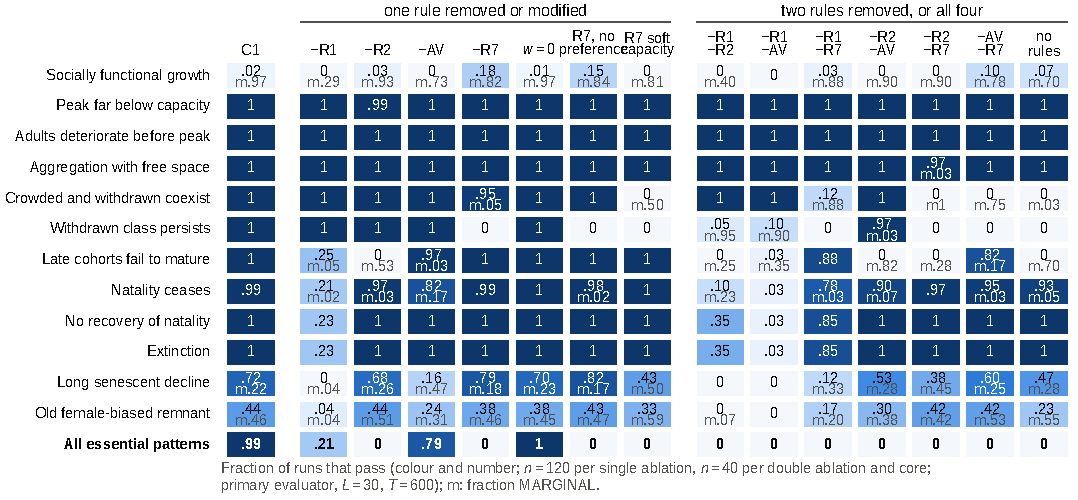
\includegraphics[width=\textwidth]{fig_em_s_ablations.pdf}
  \caption{Which pattern fails in each ablation. Fraction of runs that pass each pattern (colour and upper number) and
  fraction MARGINAL (m), for \Cone\ and its single ablations (left: without the sensitive window, R1, adults
  recovering at the juvenile rate; without social learning, R2; without crowd aversion, AV; without retreat sites,
  R7; $w=0$ with faster learning; retreat sites without preference or with soft capacity) and double ablations and
  the core model without the four social rules (right). Primary evaluator, $n=120$ per single ablation and $n=40$ per double
  ablation and for the core model, $L=30$, $T=600$. Source:
  \texttt{results\_em/pattern\_tables/ablations.csv}.}
  \label{fig:ablations}
\end{figure}



\begin{figure}[ht]
  \centering
  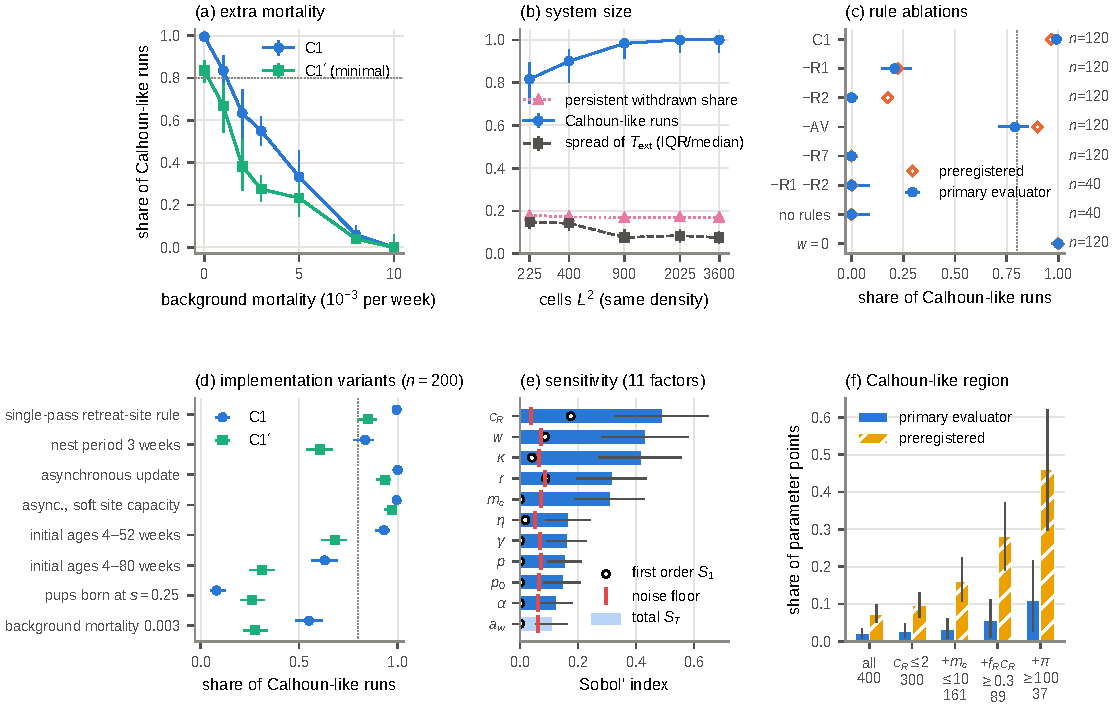
\includegraphics[width=\textwidth]{fig_em_robustness.pdf}
  \caption{Statistical robustness of the joint outcome (share of runs that pass every essential pattern
  jointly, O17p; 95\% Wilson intervals; dotted line: the 0.8 threshold fixed before the runs). (a)~Constant
  background mortality at all ages ($n=200$ at 0, 0.003 and 0.008 per week, 60 elsewhere): the outcome is lost
  through the timing of the end of natality (O5), while the patterns that discriminate against the null models pass
  at every value. (b)~Lattice size at fixed seeding density ($n=60$ per size): share of runs with the joint outcome,
  Kaplan--Meier spread of the extinction time and persistent withdrawn share. (c)~Rule ablations of \Cone, scored
  with the primary (filled) and the preregistered evaluator (open): without the sensitive window (R1), social
  learning (R2) or retreat sites (R7) the outcome is lost, without crowd aversion (AV) it falls to 0.79, and maternal
  transmission is not needed ($w=0$ with faster learning). (d)~Implementation variants and initial conditions
  ($n=200$). (e)~Sobol' indices of O17p over 11 factors (Saltelli design, $3\,328$ parameter points $\times$ 6 runs;
  \citealp{Saltelli2010}): total (bars, bootstrap intervals; pale: below the relevance criterion), first order
  (circles) and empirical noise floor (red). (f)~Share of parameter points that reproduce the joint outcome ($k/n\ge0.8$) in two
  15-factor Latin hypercubes (400 points $\times$ 10 runs), in nested subsets chosen after the runs, with bootstrap
  intervals over points.}
  \label{fig:robustness}
\end{figure}

\paragraph{Occupancy at the peak}
At the peak of the spatial \Cone\ (week 55 [54, 56], $N\approx2\,600$; 200 runs) the mean occupancy is 2.90 [2.88,
2.91] animals per cell, but the distribution is aggregated: the variance-to-mean ratio is 2.53 [2.51, 2.55], the
maximum 16.1 [15.8, 16.3] (10--90\% of runs: 14--19), and the average animal lives in a cell of 5.42 [5.40, 5.45]
animals. A fraction 0.183 [0.180, 0.187] of the animals sits in cells above the damage threshold $m_c=8$
(Fig.~\ref{fig:occupancy}). Figure~\ref{fig:snapshots} shows one colony at its peak and in its decline.

\begin{figure}[ht]
  \centering
  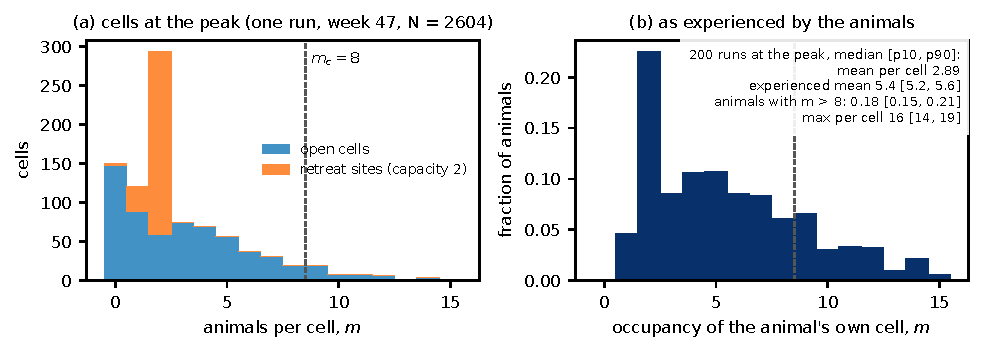
\includegraphics[width=0.85\textwidth]{fig_em_s_occupancy.pdf}
  \caption{Occupancy per cell at the peak of the spatial \Cone. (a)~Histogram of cells in one run (seed 1, week 47,
  $N=2\,604$), ordinary cells and retreat sites (capacity 2) stacked; dashed: $m_c=8$. (b)~Occupancy of the own cell
  as experienced by the animals in the same run. Inset: ensemble values at $\arg\max N$ over 200 runs (median and
  10--90\% range). Source: \texttt{results\_em/robustness\_checks/occupancy\_\{peak.json,ensemble.csv\}}.}
  \label{fig:occupancy}
\end{figure}

\begin{figure}[ht]
  \centering
  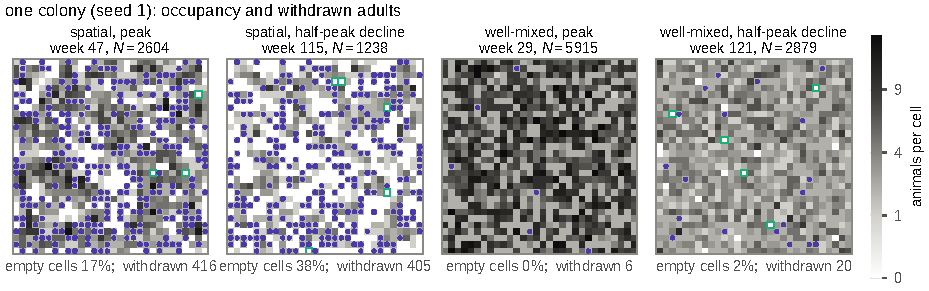
\includegraphics[width=\textwidth]{fig_em_s_snapshots.pdf}
  \caption{One colony (seed 1) at its peak and halfway down its decline, in space and well mixed with mating in the
  cell: grey, animals per cell (common square-root scale); dots, withdrawn non-breeders (adults with $s<0.2$
  isolated for at least 4 weeks; area proportional to number); squares, empty retreat sites. In space the colony
  aggregates beside empty cells (17\% and 38\% empty) and lodges a withdrawn class (416 and 405 adults); well mixed
  the occupancy is homogeneous (0\% and 2\% empty) and almost nobody stays isolated (6 and 20). A single run is
  illustrative; ensemble rates are in Fig.~5 of the main text.}
  \label{fig:snapshots}
\end{figure}

% ===========================================================================
% ===========================================================================
% Self-contained SM section, placed after "Robustness" (supp:robustness) and before "Supplementary videos".
% The tables tab_sm_*.tex are written by scripts/em/f9_sm_tablas.py (make em-tables) from results_em/.
\section{Adult recovery, mate search and colony size}
\label{supp:recovery}\label{sec:recovery}

This section gives, from archived runs, the numbers on which the
conditions of the mechanism rest (main text, Sections~3.2 and~4.2): the extinction probability as a function of adult
recovery, its dependence on colony size, the effect of removing non-breeders, of background mortality and of
protecting the juveniles, the test of a mate-finding Allee effect, the scaling of the extinction
time, the cohort-by-cohort account of the mechanism in the well-mixed limit, and the held-out patterns of the
reversible branch. Every count is reproduced by
\texttt{scripts/em/f9\_sm\_tablas.py} in the code repository.

\paragraph{Design}
The adult recovery factor $\eadult\in[0,1]$ multiplies the gain of an individual outside the window: an adult gains
$\eadult\,r[(1-\lambda)+\lambda\bar s_V]$ per week, so that with $\lambda<1$ a non-breeding adult recovers on its own
at rate $\eadult r(1-\lambda)$, and with $\lambda=1$ only from competent neighbours. \Cone\ is $\eadult=0$, $\lambda=1$.
We ran $\eadult\in\{0,0.01,0.02,0.05,0.1,0.2,0.3,0.4,0.5,0.6,0.8,1\}$ and $\lambda\in\{0,0.5,0.8,0.9,0.95,1\}$, with
all other rules of \Cone, at $L=15$ (20 replicates), $L=30$ (20) and $L=60$ (10; nine values of $\eadult$ and a
subset of $\lambda$), in space (with retreat sites) and well mixed (without retreat sites; father drawn in the
female's cell, in her $3\times3$ block or in the whole arena): $12\,870$ colonies in all, with the founders and the
seeding density of \Cone. The response is the probability of extinction by week $1\,000$, with $95\%$ Wilson
intervals \citep{Wilson1927}; for an ensemble in which every colony goes extinct the interval is $[0.84,1]$ with 20
replicates and $[0.72,1]$ with 10. The threshold $\eadult^c(\lambda,L)$ is the midpoint of a binomial
maximum-likelihood logistic fit of the extinction probability against $\eadult$.

\paragraph{Small adult recovery does not prevent the collapse}
With $\eadult\le0.02$ every colony went extinct: $2\,880$ of $2\,880$ at $L=15$ and $30$, in space and well mixed,
under the three mating rules and for every $\lambda$ (Table~\ref{tab:sm-pext}); with $\eadult=0$, every one of the
$1\,110$ colonies at $L=15$--$60$. The collapse is therefore not an artefact of the edge $\eadult=0$. It is lost
when adults recover fast enough on their own (Table~\ref{tab:sm-epsc}). At the size of the experiment ($L=30$)
the threshold is $0.085$ in space with individual recovery ($\lambda=0$) and $0.73$ in space with purely social
recovery ($\lambda=1$); well mixed it is $0.70$ for $\lambda=0$ and exceeds $1$ for $\lambda\ge0.5$ (at $\lambda=1$
every colony goes extinct even with $\eadult=1$): without competent demonstrators an adult whose recovery is social
never recovers. The relevant condition is thus that
adults do not recover \emph{asocially}, that is, that $\eadult(1-\lambda)$ is small, and in space that the pockets of
competent animals that survive the crowded phase are too few to teach the adults around them.

\begin{table}[ht]
\centering
\caption{Probability that a colony of \Cone\ with adult recovery factor $\eadult$ is extinct by week $1\,000$, for
purely social ($\lambda=1$) and purely individual ($\lambda=0$) learning and recovery, in space (with retreat sites)
and well mixed (no retreat sites, mating in the cell), at $L=15$, $30$ and $60$. $n$: replicates per cell of the
table. --: not simulated. 95\% Wilson intervals: $[0.84,1]$ for $20/20$, $[0.72,1]$ for $10/10$, at most $\pm0.22$
otherwise. Source: \texttt{results\_em/adult\_recovery/summary.csv}.}
\label{tab:sm-pext}
\scriptsize
\setlength{\tabcolsep}{2.6pt}
\begin{tabular}{@{}lcrr*{12}{c}@{}}
\toprule
& & & & \multicolumn{12}{c}{$\eadult$} \\
\cmidrule(l){5-16}
Structure & $\lambda$ & $L$ & $n$ & 0 & .01 & .02 & .05 & .1 & .2 & .3 & .4 & .5 & .6 & .8 & 1 \\
\midrule
spatial & 1 & 15 & 20 & 1 & 1 & 1 & 1 & 1 & 1 & 1 & .95 & .95 & .95 & .60 & .55 \\
spatial & 1 & 30 & 20 & 1 & 1 & 1 & 1 & 1 & 1 & .95 & .90 & .85 & .70 & .50 & .05 \\
spatial & 1 & 60 & 10 & 1 & -- & -- & 1 & 1 & .90 & 1 & .80 & -- & .40 & 0 & 0 \\
\addlinespace
spatial & 0 & 15 & 20 & 1 & 1 & 1 & 1 & .80 & .05 & 0 & 0 & 0 & 0 & 0 & 0 \\
spatial & 0 & 30 & 20 & 1 & 1 & 1 & .85 & .30 & 0 & 0 & 0 & 0 & 0 & 0 & 0 \\
spatial & 0 & 60 & 10 & 1 & -- & -- & .50 & 0 & 0 & 0 & 0 & -- & 0 & 0 & 0 \\
\addlinespace
well mixed & 1 & 15 & 20 & 1 & 1 & 1 & 1 & 1 & 1 & 1 & 1 & 1 & 1 & 1 & 1 \\
well mixed & 1 & 30 & 20 & 1 & 1 & 1 & 1 & 1 & 1 & 1 & 1 & 1 & 1 & 1 & 1 \\
well mixed & 1 & 60 & 10 & 1 & -- & -- & 1 & 1 & 1 & 1 & 1 & -- & 1 & 1 & 1 \\
\addlinespace
well mixed & 0 & 15 & 20 & 1 & 1 & 1 & 1 & 1 & 1 & 1 & 1 & 1 & 1 & .65 & 0 \\
well mixed & 0 & 30 & 20 & 1 & 1 & 1 & 1 & 1 & 1 & 1 & 1 & 1 & 1 & 0 & 0 \\
well mixed & 0 & 60 & 10 & 1 & -- & -- & 1 & 1 & 1 & 1 & 1 & -- & .60 & 0 & 0 \\
\bottomrule

\end{tabular}
\end{table}

\begin{table}[ht]
\centering
\caption{Threshold of adult recovery $\eadult^c(\lambda,L)$ above which the colony persists: midpoint of the logistic
fit of the extinction probability by week $1\,000$ against $\eadult$. In brackets, where computed, the
profile-likelihood 95\% interval of the midpoint (width of the sigmoid profiled out; $>1$: beyond the grid).
$^\ast$Only one value of $\eadult$ gives an intermediate extinction fraction, so the width of the transition is not
identified. $^\dagger$No intermediate value: the threshold lies between the last $\eadult$ at which every colony goes
extinct and the first at which none does. $>1$: every colony goes extinct even with $\eadult=1$, or the fitted
midpoint exceeds 1. n.s.: not simulated. In space with retreat sites; well mixed without them. Sources:
\texttt{results\_em/adult\_recovery/transicion.csv} and
\texttt{results\_em/robustness\_checks/epsc\_profile.csv}.}
\label{tab:sm-epsc}
\footnotesize
\begin{adjustbox}{max width=\textwidth}
\begin{tabular}{@{}lcccc@{}}
\toprule
Structure and mating & $\lambda$ & $L=15$ & $L=30$ & $L=60$ \\
\midrule
spatial & 0 & 0.133 [0.113, 0.157] & 0.085 [0.073, 0.099] & 0.050 [0.037, 0.063]$^\ast$ \\
spatial & 0.5 & 0.22 & 0.17 & n.s. \\
spatial & 0.8 & 0.34 & 0.26 & n.s. \\
spatial & 0.9 & 0.46 [0.43, 0.50] & 0.38 [0.35, 0.42] & 0.31 [0.27, 0.35] \\
spatial & 0.95 & 0.54 & 0.48 & n.s. \\
spatial & 1 & 0.97 [0.88, $>1$] & 0.73 [0.67, 0.81] & 0.53 [0.46, 0.62] \\
\addlinespace
well mixed, cell & 0 & 0.80 [0.79, 0.86]$^\ast$ & 0.6--0.8$^\dagger$ & 0.60 [0.57, 0.67]$^\ast$ \\
well mixed, cell & 0.5 & $>1$ & $>1$ & $>1$ \\
well mixed, cell & 1 & $>1$ & $>1$ & $>1$ \\
\addlinespace
well mixed, $3\times3$ block & 0 & 0.84 & 0.60 & 0.58 \\
well mixed, $3\times3$ block & 0.5 & $>1$ & 0.91 & 0.70 \\
well mixed, $3\times3$ block & 1 & $>1$ & $>1$ & $>1$ \\
\addlinespace
well mixed, global & 0 & 0.81 [0.76, 0.86] & 0.51 [0.48, 0.54] & 0.30 [0.27, 0.33]$^\ast$ \\
well mixed, global & 0.5 & $>1$ & 0.69 & 0.40 \\
well mixed, global & 1 & $>1$ & $>1$ & $>1$ \\
\bottomrule

\end{tabular}
\end{adjustbox}
\end{table}

\paragraph{The tolerated recovery decreases with colony size}
In space the threshold decreases with $L$ for every $\lambda$, with no sign of saturation between $L=15$ and $60$:
with $\lambda=0$ it is $0.133$ [$0.113$, $0.157$], $0.085$ [$0.073$, $0.099$] and $0.050$ [$0.037$, $0.063$] at $L=15$,
30 and 60, and with $\lambda=1$ it is $0.97$ [$0.88$, $>1$], $0.73$ [$0.67$, $0.81$] and $0.53$ [$0.46$, $0.62$]
(profile-likelihood 95\% intervals of the midpoint of a binomial logistic fit; for $\lambda=0$ and $1$ the intervals
for different $L$ do not overlap; for $\lambda=0.9$ those for $L=30$ and $60$, $[0.347, 0.420]$ and $[0.273, 0.349]$,
overlap by $0.002$; likelihood-ratio $p\le0.008$ for every pair of sizes, also for $\lambda=0.9$). The width of the transition is not
identified at $L=60$, where only one or two values of $\eadult$ give an intermediate extinction fraction, and a
common width for the three sizes is not rejected ($p=0.26$, $0.11$ and $0.12$ for $\lambda=0$, $0.9$ and $1$), so the
data do not show whether the transition sharpens. Three sizes do not determine the limit of the threshold as
$L\to\infty$, which may be zero.
For any $\eadult>0$ the spatial collapse may therefore be a finite-size effect; only the edge $\eadult=0$ is
supported at every size simulated ($270$ of $270$ spatial colonies at $L=15$--$60$). Well mixed with mating in the
cell the series ($0.80$, between $0.6$ and $0.8$, and $0.60$ for $\lambda=0$) is resolved only to the grid of
$\eadult$ (likelihood-ratio $p=0.16$ and $1.0$ for the pairs of sizes); it is compatible with the value of the
deterministic limit, $0.585$, at which the deterministic orbit acquires an attracting invariant curve, but does not
show convergence to it. With global mating it decreases fast ($0.81$, $0.51$, $0.30$, non-overlapping intervals) and
that limit is close to zero. The conclusion of the main text is
conditional on the scale of the experiment for this reason: a much larger closed colony would need an even less
reversible non-breeding state.

\paragraph{A measurable indicator of the outcome}
Late breeding, the fraction of adults of breeding age that conceive from 30 weeks after the end of natality, is at
most $0.008$ in 90\% of the 819 spatial colonies that die out and at least $0.087$ in 90\% of the 621 that persist
(area under the ROC curve $0.97$; $0.99$ for $\lambda=1$; well mixed $0.99$, with a 10th percentile of $0.017$ in the
42 colonies that persist), over the sweep of $\eadult\times\lambda$ at $L=30$. Source:
\texttt{results\_em/operational\_indicators/tabla\_auc.csv}.

\paragraph{Held-out patterns of the reversible branch}
The two patterns of earlier confined colonies scored on the reversible-suppression null (main text, Section~3.2) were
defined after the production runs. The null ($\eadult=0.8$, $\lambda=0.9$, $L=30$, 200 runs) and \Cone\ were re-run
bit for bit with the archived seeds to record every litter. Each run is split into four windows: \emph{growth}, from
week 10 to the entry into the plateau; \emph{plateau}, the weeks with $N\ge0.9\,N_{\max}$ contiguous to the maximum
(median weeks 34 to about 100); \emph{decline}, from the end of the plateau to the following trough (median week
141); and \emph{late}, weeks $\ge300$. \emph{Litter loss}: a litter fails when none of its pups survives; the
fraction of failed litters is computed exactly from the litter record in each window. The weekly births per
reproductive female factor exactly as $B=C\,\bar\ell\,\varphi$ (conception rate, mean litter size at conception, a constant of the model, and
mean pup survival), so the fall of natality from growth to plateau splits additively on a logarithmic scale; the share of
conception is $\ln(C_{\rm g}/C_{\rm p})/[\ln(C_{\rm g}/C_{\rm p})+\ln(\varphi_{\rm g}/\varphi_{\rm p})]$. The null gives failed litters $0.048$ [$0.046$, $0.050$] during growth, $0.243$ [$0.239$, $0.248$] on
the plateau, $0.073$ [$0.067$, $0.079$] in the decline and $0.102$ [$0.101$, $0.102$] late (\Cone: $0.026$ and $0.087$
during growth and on the plateau); conception falls $8.4$-fold and pup survival $2.15$-fold, a conception share of
$0.73$ [$0.73$, $0.74$]. \emph{Females that never breed}: the fraction of the females born in a window that do not
conceive by 48 weeks of age, those that die earlier counting as never breeding (the definition of O11b). It is
$0.889$ [$0.885$, $0.893$] for females born on the plateau of the null ($41\,202$ females) against $0.961$ [$0.958$,
$0.964$] in \Cone, $0.366$ [$0.356$, $0.376$] for those born in the decline and $0.719$ [$0.718$, $0.720$] for those born
from week 300 (to $T-48$); in \Cone\ no female is born after the plateau. Means over runs with bootstrap 95\%
intervals. Source: \texttt{results\_em/robustness\_checks/h2h3.json}, from
\texttt{\{rev1000,c1x\}\_\{litters,cohorts\}.csv} (scripts \texttt{f10\_reversible.py} and \texttt{f10\_h2h3.py}).

\paragraph{Removal of non-breeders, background mortality and protection of juveniles}
These experiments use \Cone\ at $L=30$, in space with retreat sites and well mixed without them, with a horizon of
$1\,500$ weeks (removal) or $1\,000$ weeks (mortality). \emph{Single removal.} At week $t_r$ a fraction $f$ of the
adults with $s<s_v$ is removed at random ($f\in\{0.25,0.5,0.75,0.9,1\}$; $t_r$ from 20 to 100 weeks in space and from
15 to 50 well mixed; 20 replicates per cell). It delays extinction but does not prevent it: $12$ of $1\,000$ spatial
colonies (all with $f\ge0.9$ and $t_r=30$--$60$) and $0$ of $900$ well-mixed ones were alive at week $1\,500$; the
median extinction time rises at most from $163$ to $761$ weeks in space and from $148.5$ to $272$ well mixed. Removing
instead the adults that did not breed in the previous 8 weeks, once, gives $3$ survivors of $240$. \emph{Sustained
removal.} Removing $25\%$ or $50\%$ of the non-breeders every four weeks from $t_r=30$ keeps $20$ of $20$ spatial colonies
alive at week $1\,500$; well mixed, removing $50\%$ from $t_r=20$, 25 or 30 does the same, and $25\%$ rescues $10$--$11$
of $20$ from $t_r=20$--$25$ and none from $t_r=30$. Starting later rescues fewer ($t_r=50$ in space: $4$ and $15$ of
$20$). If the removal stops after 52, 104 or 208 weeks the colony collapses again: $2$ of $60$ spatial and $0$ of $60$
well-mixed colonies were alive at week $1\,500$. \emph{Background mortality.} An extra weekly mortality $\mu_{\rm bg}$,
independent of age and state, does not rescue \Cone: $10$ of $10$ colonies went extinct at each
$\mu_{\rm bg}\in\{0.005,0.01,0.02,0.03,0.05\}$, in space and well mixed. It rescues only when competence can
regenerate: with asocial learning ($\lambda=0$, $\eadult=0$) from $\mu_{\rm bg}=0.02$ in space ($10$ of $10$ alive) and
$0.05$ well mixed, and with $\lambda=0.9$, $\eadult=0.3$ from $0.01$ in space and $0.03$ well mixed. \emph{Protection
of juveniles.} From week $t_1\in\{15,20,25,30,40\}$, for 12, 26 or 52 weeks or permanently, the juveniles in their
window either learned from perfect demonstrators ($\bar s_V:=1$) or suffered no crowding damage (a crowding-free
nursery); 10 replicates per cell. Of the $800$ manipulated colonies $798$ went extinct; the two survivors had perfect
demonstrators permanently from week 30 or 40, in space. The median extinction time moved by at most $159$ weeks in
space and $12$ well mixed. Sources: \texttt{results\_em/hydra\_removal/summary.csv},
\texttt{results\_em/background\_mortality/summary.csv} and \texttt{results\_em/juvenile\_protection/tabla\_p3.csv}.

\paragraph{Not a mate-finding Allee effect}
In the reference model a female conceives only with a male of her own cell. Well mixed, with $\lambda=1$ and
$\eadult=0$, \Cone\ went extinct in every colony under the three mating rules, $50$ of $50$ under each
(Table~\ref{tab:sm-mate}); global mating makes the collapse earlier, not rarer. The short-lived control (SL), whose
competence regenerates individually, also dies out well mixed with mating in the cell or in the block, but with
global mating it persists for $L\ge45$ (none of $60$ colonies extinct by week $3\,000$, and no late extinction in $1.6\cdot10^5$
colony-weeks). Under perfect mate search the well-mixed variant therefore separates the two
models: the social collapse of \Cone\ does not depend on mate finding, whereas the extinction of the well-mixed SL with
local mating does.

\begin{table}[ht]
\centering
\caption{Well-mixed \Cone\ ($\lambda=1$, $\eadult=0$, no retreat sites; horizon $2\,000$ weeks) and the short-lived
control SL (horizon $3\,000$ weeks) with the father drawn in the female's cell, in her $3\times3$ block or in the
whole arena. Extinct/replicates at each $L$ (\Cone: $L=15$, $30$, $60$; SL: $L=10$, 15, 20, 30, 45, 60, 90, and 120
with global mating), the pooled count with its $95\%$ Wilson interval when every colony went extinct, the probability
of extinction by week 300 at each $L$, and the range of the median extinction time over $L$ (weeks). Source:
\texttt{results\_em/mate\_search/tabla\_mate.csv}.}
\label{tab:sm-mate}
\scriptsize
\setlength{\tabcolsep}{3pt}
\begin{adjustbox}{max width=\textwidth}
\begin{tabular}{@{}llllllc@{}}
\toprule
Model & Mating & $L$ & Extinct / replicates & Pooled & $P(\text{extinct by }300)$ & median $T_{\rm ext}$ \\
\midrule
\textsf{C1} & cell & 15--60 & 20/20, 20/20, 10/10 & 50/50 [0.93, 1.00] & 1, 1, 1 & 147--150 \\
\textsf{C1} & $3\times3$ block & 15--60 & 20/20, 20/20, 10/10 & 50/50 [0.93, 1.00] & 1, 1, 1 & 139--143.5 \\
\textsf{C1} & global & 15--60 & 20/20, 20/20, 10/10 & 50/50 [0.93, 1.00] & 1, 1, 1 & 138--141.5 \\
\addlinespace
\textsf{SL} & cell & 10--90 & 30/30, 30/30, 30/30, 30/30, 20/20, 20/20, 10/10 & 170/170 [0.98, 1.00] & 1, 1, 1, 1, 1, 1, 1 & 86.5--128.5 \\
\textsf{SL} & $3\times3$ block & 10--90 & 30/30, 30/30, 30/30, 30/30, 20/20, 20/20, 10/10 & 170/170 [0.98, 1.00] & 1, 1, 1, 1, 1, 1, 1 & 78--125.5 \\
\textsf{SL} & global & 10--120 & 30/30, 30/30, 30/30, 24/30, 0/20, 0/20, 0/10, 0/10 & -- & .93, .87, .47, .20, 0, 0, 0, 0 & 76--1070.5 \\
\bottomrule

\end{tabular}
\end{adjustbox}
\end{table}

\paragraph{Extinction is certain; its scaling distinguishes collapse from persistence}
Competence is updated before reproduction and the damage $\gamma(m_i-m_c)_+$ exceeds $1+r$ above an occupancy
$\bar m=m_c+(1+r)/\gamma$, so no animal in a cell with more than $\bar m$ occupants can breed; a pigeonhole argument
then bounds the females that can conceive in a week by a multiple of $|G|$. With no immigration, extinction of a closed
colony is certain for every variant with $\gamma>0$ (a standard argument for a population with an absorbing empty
state and a bounded number of breeders). The
fact that \Cone\ goes extinct in 200 of 200 runs is therefore informative only through the time scale. A collapse
has an extinction time that grows like $\ln|G|$; a metastable colony one that grows like $e^{c|G|}$. Both behaviours
are observed. With $\eadult=0$ the median extinction time of \Cone\ grows by $1$--$2$ weeks per unit of $\ln|G|$ well
mixed (all mating rules) and by about $6$ ($\lambda=0$) and $11$ ($\lambda=1$) weeks in space, with noisier values
between, where the last pockets die later in larger arenas (\texttt{escaleo.csv}); over the well-mixed ensembles of $L=10$--$250$ the slope is $1.25$ [$1.16$, $1.33$] weeks per
unit of $\ln N_0$, and the median residual time from the last birth to extinction is $115$--$118$ weeks at every size
(\texttt{results\_em/wellmixed\_size\_scaling/tabla\_wm.csv}). On the persistent side of the threshold the extinction probability falls with size
(space, $\lambda=1$, $\eadult=1$: $0.55$, $0.05$ and $0$ at $L=15$, $30$ and $60$), and the spatial SL is metastable,
with a late extinction rate that decreases like $e^{-c|G|}$, $c\approx0.005$ per cell. The answer to ``is the collapse
a consequence of the small size of the colony?'' is thus negative for $\eadult=0$, where the time to extinction grows
only logarithmically with size, and open for $\eadult>0$ in space, where the tolerated recovery decreases with size.

\paragraph{The mechanism cohort by cohort in the well-mixed limit}
As $|G|\to\infty$ at fixed density the well-mixed model approaches a deterministic kinetic equation for the
density of individuals by age and competence: at $L=90$ the largest difference between its density and the mean of the
simulations is $0.19\%$ of the peak (\texttt{results\_em/kinetic/resumen\_kin\_vs\_abm\_L90.csv}).
Along its orbit for \Cone\ the density $\nu$ of other individuals per cell exceeds $\nu^*=6.92$, the occupancy at which
the expected damage $\gamma\,\mathrm{E}(\mathrm{Poisson}(\nu)+1-m_c)_+$ equals the maximal gain $r$, from week 25 to
week 108. Table~\ref{tab:sm-cohorts} follows five cohorts. Their competence at the end of the window, relative to
that of their mothers, collapses between the cohorts of weeks 12 and 22, while the mean proportion $\bar\theta$ of
neighbours with $s>0$ during their window is still above the transmission threshold $\theta^*=(1-w)/(ra_w)=2/3$ for
all but the last, and while a gain bound that ignores damage would still predict ratios of $0.63$--$0.90$. The cohorts
thus fail through damage inside the window, not through a lack of demonstrators. That a sustained density above
$\nu^*$ \emph{implies} the collapse is a conjecture, verified at every point of the bifurcation diagram of the kinetic
equation but not proved. This account holds for the well-mixed model. In space the
mean crowding is far below $\nu^*$ (2.9 animals per cell at the peak), the crowding experienced by juveniles exceeds
the maximal gain only during the growth phase, and the colony collapses because the adults, damaged during the
aggregated growth and unable to recover, become non-breeding: an adult ratchet, which is why adult recovery decides
the outcome.

\begin{table}[ht]
\centering
\caption{Cohorts of the kinetic (well-mixed, deterministic) limit of \Cone. $b$: week of birth. Ratio: mean competence
of the cohort at the end of its window ($a=13$) over that of its mothers. $\bar\theta$: mean, over the window weeks
$b+1,\dots,b+12$, of the proportion of neighbours with $s>0$. Bound without damage: the ratio that the mean-field gain
alone would give. Last column: $\bar\theta\ge\theta^*=2/3$. Source:
\texttt{results\_em/kinetic/cohortes\_C1.csv}.}
\label{tab:sm-cohorts}
\footnotesize
\begin{tabular}{@{}ccccc@{}}
\toprule
$b$ & ratio & $\bar\theta$ & bound without damage & $\bar\theta\ge\theta^*$ \\
\midrule
3 & 0.991 & 1.00 & 1.02 & yes \\
12 & 0.718 & 1.00 & 0.90 & yes \\
16 & 0.188 & 0.94 & 0.77 & yes \\
19 & 0.0301 & 0.82 & 0.63 & yes \\
22 & 0.00419 & 0.63 & 0.48 & no \\
\bottomrule

\end{tabular}
\end{table}

\paragraph{Status of the claims}
The claims of the main text about the mechanism have different status. Definitions: $\nu^*=6.92$ and $\theta^*=2/3$,
computed exactly. Short argument: extinction of a closed colony is certain for $\gamma>0$ (see above; uninformative
about time scales). Conjectural: that a density above $\nu^*$ during the window implies the collapse (verified
numerically in the kinetic equation). Simulated: the level of the peak, $0.36\Kg$; growth to the numerical cap without
crowding damage (200 of 200 spatial runs); the collapse for $\eadult\le0.02$ and the threshold $\eadult^c(L)$, whose
limit $L\to\infty$ is not determined (Tables~\ref{tab:sm-pext}--\ref{tab:sm-epsc}); the effects of removing
non-breeders, of background mortality and of protecting the juveniles; the absence of a mate-finding Allee effect,
well mixed (Table~\ref{tab:sm-mate}); the logarithmic growth of the extinction time; the crossing of $\theta^*$
before the end of natality, also in colonies that persist; and the spatial mechanism, an adult ratchet during the
aggregated growth.


% ===========================================================================
\section{Supplementary videos}
\label{supp:videos}

The videos are supplied as separate MP4 files (1280$\times$720 pixels, 12 frames per second, one frame every two
weeks); they are also in \texttt{results/movies/} of the code repository, with the script that regenerates them.
Each shows one run ($L=30$, seed 1, the colony of Fig.~\ref{fig:snapshots}). Left panel: animals per cell (grey,
square-root scale common to all models); magenta dots: withdrawn non-breeders (adults with $s<0.2$ isolated, at most
two animals in the cell, for at least four consecutive weeks; dot area proportional to their number); blue squares:
retreat sites. Right panel: fraction of competent animals ($s\ge0.2$) per cell. Bottom: $N(t)$ with a cursor, the
phases A--D dated as in Fig.~2 of the main text, and the number of withdrawn non-breeders. A single run is
illustrative; ensemble statistics are in the main text.

\paragraph{Video S1} (\texttt{video\_S1\_comparison.mp4}). Synchronised mosaic of the spatial \Cone, the well-mixed
\Cone\ (mating in the cell, retreat sites acting only as a capacity), the short-lived control and the core model
without the four social rules, weeks 0--600.

\paragraph{Video S2} (\texttt{video\_S2\_C1\_spatial.mp4}). The spatial \Cone, from the founders to extinction.

\paragraph{Video S3} (\texttt{video\_S3\_C1\_wellmixed.mp4}). The well-mixed \Cone, from the founders to extinction.

\bibliographystyle{elsarticle-harv}
\bibliography{refs}

\end{document}
